\chapter{Grundlagen}
\label{kap2}

\section{Laufroboter}

\subsection{Lauron}

Die erste Version des Lauron (Laufender Roboter Neuronal gesteuert) wurde 1994 am Forschungszentrum für Informatik (FZI) in Karlsruhe \autocite{fzi} entwickelt. Zunächst war es das Ziel Laufmuster durch neuronale Netze zu entwickeln und zu testen.

Die zweite Version des Lauron verbessert die Sensorausstattung sowie die Mechanik des Laufroboters. Des Weiteren wurde das Steuerungsprinzip, das auf neuronalen Netzen basierte, durch die hierarichische MCA-Architektur \autocite{scholl2001modular} ausgetauscht. 

\begin{figure}[b!]
  \centering
  \begin{subfigure}[b]{.4\linewidth}
    \centering
    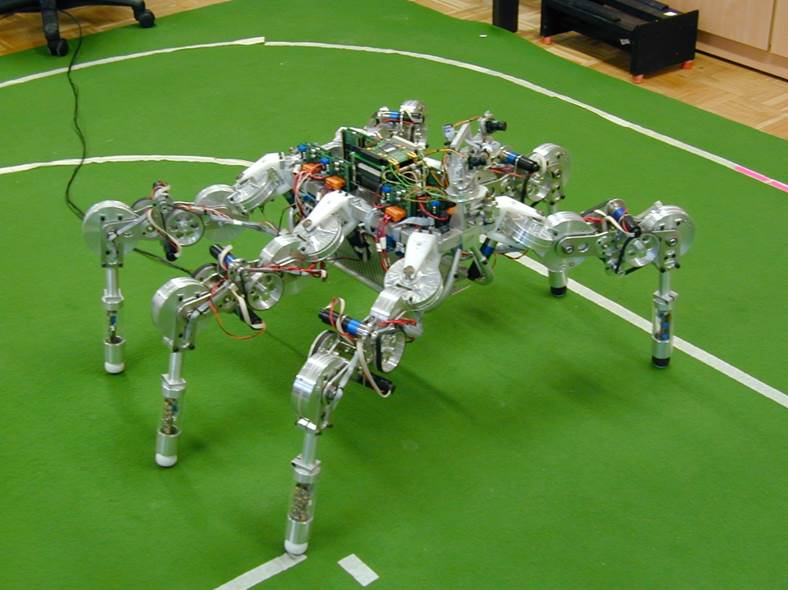
\includegraphics[width=6cm]{kapitel2/lauron3}
    \subcaption{Lauron III}\label{kap2:lauron3}
  \end{subfigure}%
  \qquad
  \begin{subfigure}[b]{.4\linewidth}
    \centering
    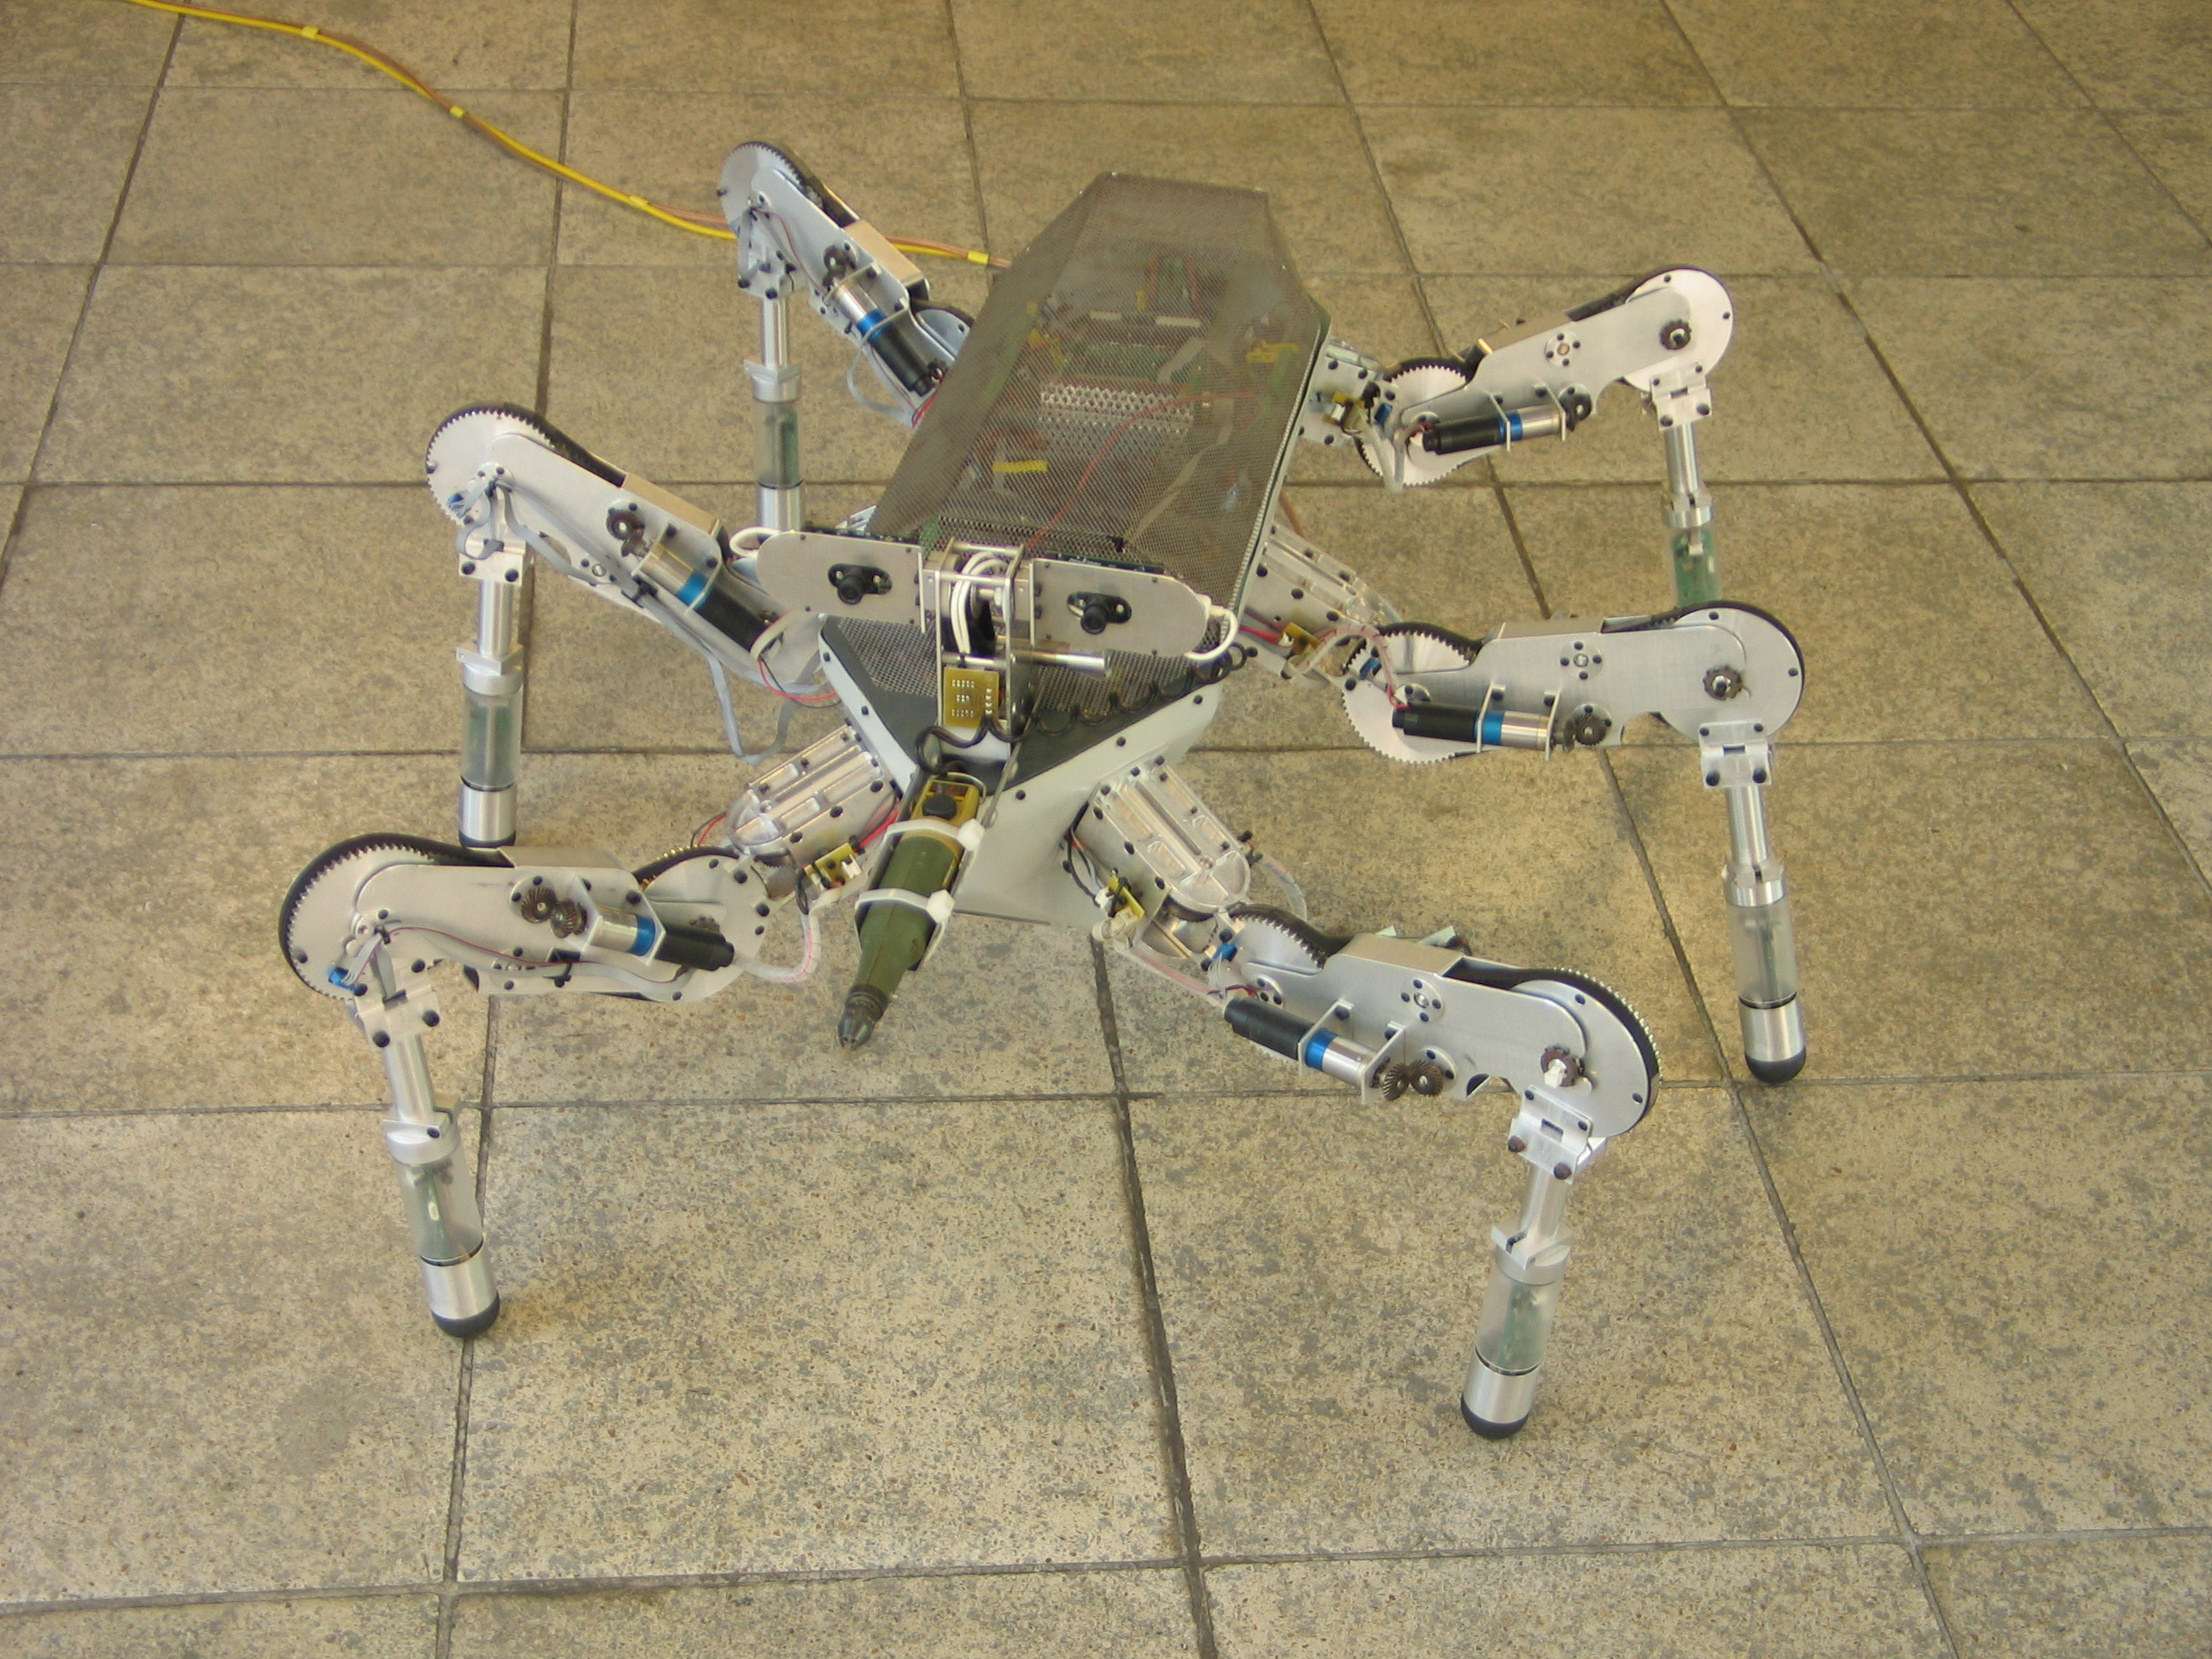
\includegraphics[width=6cm]{kapitel2/lauronivb}
    \subcaption{Lauron IVb}\label{kap2:lauron4b}
  \end{subfigure}\\
  \caption{Verschiedene Versionen des Lauron}
  \label{kap2lauron}
\end{figure}

Für die dritte Version \emph{Lauron III} existiert der vorliegende Laufplaner. Daher wird nun näher auf diese Version des Laufroboters sowie auf den grundlegende Konzept des Lauron eingegangen. Eine weitere Version des Laufroboters ist der \emph{Lauron IVb}, welcher sich an der Hochschule Mannheim befindet. Die neuste Version des Laufroboters ist der \emph{Lauron V}.

\subsubsection{Indische Stabheuschrecke als Vorbild}

Der Lauron basiert auf dem Vorbild der indischen Stabheuschrecke (Carausius morosus), die sehr gut erforscht ist. Dies gilt sowohl für den mechanischen Aufbau als auch für die Abläufe der Bewegungen des Roboters. Der Körper ist in drei Teile geteilt, von denen die Brust wiederum in drei Teile für jeweils ein Beinpaar unterteilt sind.
\begin{itemize}
  \item Kopf (Caput)
  \item Brust (Thorax)
  \begin{itemize}
  \item Hüfte (Coxa)
  \item Oberschenkel (Femur)
  \item Unterschenkel (Tibia)
  \end{itemize}
  \item Hinterleib (Abdomen)
\end{itemize}

Die Segmente sind durch die Gelenke Subcoxal, Coxa-Trochanter und Femur-Tibia verbunden. Der Fuß jedes Beins wird Tarsus genannt. Das erste Gelenk Subcoxal besitzt zwei Freiheitsgrade, die weiteren Gelenke besitzen ein Freiheitsgrad. Damit ist für die indische Stabheuschrecke die minimale erforderliche Zahl an Freiheitsgraden erreicht, damit der Fuß beliebig im Raum gesetzt werden kann.

Unter anderem ist noch wichtig, dass der Kopf zwei lange Fühler besitzt. Diese könnten in einem Roboter ferner  als Laserscanner oder Kamera modelliert werden, um sich einen Überblick über die Gegend verschaffen zu können. \autocite{gassmann2000} \autocite{troilo2007}

\subsubsection{Aufbau des Lauron III}

Der Körper des \emph{Lauron III} trägt die Microcontroller, die Recheneinheit, die Akkumulatoren sowie den Kamerakopf. An beiden Seiten des Körpers sind jeweils drei Beine angebracht. Der Roboter wiegt 16kg und hat eine maximale Zuladung von etwa 15kg. Die Maximalgeschwindigkeit beträgt \SI{0.5}{\metre\per\second}. \autocite{gassmann2000}

\subsection{Akrobat}

todo

\begin{figure}[t]
  \centering
  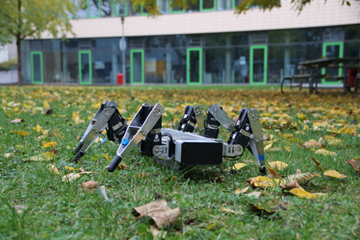
\includegraphics[height=8cm]{kapitel2/akrobat}
  \caption{Der Akrobat vor dem C-Gebäude der Hochschule Mannheim}
  \label{Kap2:akrobat}
\end{figure}



\section{Robotik}

\subsection{Koordinatensysteme}
\subsection{Direkte Kinematik}

- Mit gegebener Stellung der Gelenke Position und Orientierung des Endeffektes zu berechnen
- Transformationsmatrix, die dann aufgelöst wird und berechnet werden kann

fellmann zitieren

\autocite{fellmann2007}

\subsection{Inverse Kinematik}

- Durch Position und Orientierung des Endeffektes mögliche Stellung der Gelenke zu berechnen (meist mehrere Lösungen)
- analytische Berechnung
- numerische Berechnung: lineare Annäherung durch Jacobi-Matrix

fellmann zitieren

\autocite{fellmann2007}

\subsection{Laufplanung}

statische Laufalgorithmen, reaktive, planende Laufalgorithmen like RandomSampling

\section{Frameworks}

\subsection{Robot Operating System}
\subsection{Gazebo}
\subsection{MeshLab}